\documentclass[handout]{beamer}
%\documentclass[]{beamer}
%\usepackage[dvips]{color}
\usepackage{graphicx}
\usepackage{amsmath,amssymb,array,comment,eucal,url}
\newcommand{\e}{\mathbf{e}}
\renewcommand{\P}{\mathbf{P}}
\newcommand{\F}{\mathbf{F}}
\newcommand{\R}{\textsf{R}}
\newcommand{\mat}[1] {\mathbf{#1}}
%\newcommand{\ind}{\mathrel{\mathop{\sim}\limits^{\mathit{ind}}}}
%\newcommand{\iid}{\mathrel{\mathop{\sim}\limits^{\mathit{iid}}}}
\newcommand{\E}{\textsf{E}}
\newcommand{\SE}{\textsf{SE}}
\newcommand{\SSE}{\textsf{SSE}}
\newcommand{\RSS}{\textsf{RSS}}
\newcommand{\FSS}{\textsf{FSS}}
\renewcommand{\SS}{\textsf{SS}}
\newcommand{\MSE}{\textsf{MSE}}
\newcommand{\SSR}{\textsf{SSR}}
\newcommand{\Be}{\textsf{Beta}}
\newcommand{\St}{\textsf{St}}
%\newcommand{\C}{\textsf{C}}
\newcommand{\GDP}{\textsf{GDP}}
\newcommand{\NcSt}{\textsf{NcSt}}
\newcommand{\Bin}{\textsf{Bin}}
\newcommand{\NB}{\textsf{NegBin}}
\renewcommand{\NG}{\textsf{NG}}
\newcommand{\N}{\textsf{N}}
\newcommand{\Ber}{\textsf{Ber}}
\newcommand{\Poi}{\text{Poi}}
\newcommand{\Gam}{\textsf{Gamma}}
\newcommand{\BB}{\textsf{BB}}
\newcommand{\Gm}{\textsf{G}}
\newcommand{\Un}{\textsf{Unif}}
\newcommand{\Ex}{\textsf{Exp}}
\newcommand{\DE}{\textsf{DE}}
\newcommand{\tr}{\textsf{tr}}
\newcommand{\cF}{{\cal{F}}}
\newcommand{\cL}{{\cal{L}}}
\newcommand{\cI}{{\cal{I}}}
\newcommand{\cB}{{\cal{B}}}
\newcommand{\cP}{{\cal{P}}}
\newcommand{\bbR}{\mathbb{R}}
\newcommand{\bbN}{\mathbb{N}}
\newcommand{\pperp}{\mathrel{{\rlap{$\,\perp$}\perp\,\,}}}
\newcommand{\OFP}{(\Omega,\cF, \P)}
\newcommand{\eps}{\boldsymbol{\epsilon}}
\newcommand{\1}{\mathbf{1}_n}
\newcommand{\gap}{\vspace{8mm}}
\newcommand{\ind}{\mathrel{\mathop{\sim}\limits^{\rm ind}}}
\newcommand{\simiid}{\ensuremath{\mathrel{\mathop{\sim}\limits^{\rm
iid}}}}
\newcommand{\eqindis}{\ensuremath{\mathrel{\mathop{=}\limits^{\rm D}}}}
\newcommand{\iid}{\textit{i.i.d.}}
\newcommand{\SSZ}{S_{zz}}
\newcommand{\SZW}{S_{zw}}
\newcommand{\Var}{\textsf{Var}}
\newcommand{\corr}{\textsf{corr}}
\newcommand{\diag}{\textsf{diag}}
\newcommand{\var}{\textsf{var}}
\newcommand{\Cov}{\textsf{Cov}}
\newcommand{\Sam}{{\cal S}}
\def\H{\mathbf{H}}
\newcommand{\I}{\mathbf{I}}
\newcommand{\Y}{\mathbf{Y}}
\newcommand{\tY}{\tilde{\mathbf{Y}}}
\newcommand{\Yhat}{\hat{\mathbf{Y}}}
\newcommand{\Yobs}{\mathbf{Y}_{{\cal S}}}
\newcommand{\barYobs}{\bar{Y}_{{\cal S}}}
\newcommand{\barYmiss}{\bar{Y}_{{\cal S}^c}}
\def\bv{\mathbf{b}}
\def\X{\mathbf{X}}
\def\tX{\tilde{\mathbf{X}}}
\def\x{\mathbf{x}}
\def\xbar{\bar{\mathbf{x}}}
\def\Xbar{\bar{\mathbf{X}}}
\def\Xg{\mathbf{X}_{\boldsymbol{\gamma}}}
\def\Ybar{\bar{\Y}}
\def\ybar{\bar{y}}
\def\y{\mathbf{y}}
\def\Yf{\mathbf{Y_f}}
\def\W{\mathbf{W}}
\def\L{\mathbf{L}}
\def\w{\mathbf{w}}
\def\U{\mathbf{U}}
\def\V{\mathbf{V}}
\def\Q{\mathbf{Q}}
\def\Z{\mathbf{Z}}
\def\z{\mathbf{z}}
\def\v{\mathbf{v}}
\def\u{\mathbf{u}}

\def\zero{\mathbf{0}}
\def\one{\mathbf{1}}
\newcommand{\taub}{\boldsymbol{\tau}}
\newcommand{\betav}{\boldsymbol{\beta}}
\newcommand{\alphav}{\boldsymbol{\alpha}}
\newcommand{\A}{\mathbf{A}}
\def\a{\mathbf{a}}
\def\K{\mathbf{K}}
\newcommand{\B}{\mathbf{B}}
\def\b{\boldsymbol{\beta}}
\def\bhat{\hat{\boldsymbol{\beta}}}
\def\btilde{\tilde{\boldsymbol{\beta}}}
\def\tb{\tilde{\boldsymbol{\beta}}}
\def\bg{\boldsymbol{\beta_\gamma}}
\def\bgnot{\boldsymbol{\beta_{(-\gamma)}}}
\def\mub{\boldsymbol{\mu}}
\def\tmub{\tilde{\boldsymbol{\mu}}}
\def\muhat{\hat{\boldsymbol{\mu}}}
\def\t{\boldsymbol{\theta}}
\def\tk{\boldsymbol{\theta}_k}
\def\tj{\boldsymbol{\theta}_j}
\def\Mk{\boldsymbol{{\cal M}}_k}
\def\M{\boldsymbol{{\cal M}}}
\def\Mj{\boldsymbol{{\cal M}}_j}
\def\Mi{\boldsymbol{{\cal M}}_i}
\def\Mg{{\boldsymbol{{\cal M}_\gamma}}}
\def\Mnull{\boldsymbol{{\cal M}}_{N}}
\def\gMPM{\boldsymbol{\gamma}_{\text{MPM}}}
\def\gHPM{\boldsymbol{\gamma}_{\text{HPM}}}
\def\Mfull{\boldsymbol{{\cal M}}_{F}}
\def\tg{\boldsymbol{\theta}_{\boldsymbol{\gamma}}}
\def\g{\boldsymbol{\gamma}}
\def\eg{\boldsymbol{\eta}_{\boldsymbol{\gamma}}}
\def\G{\mathbf{G}}
\def\cM{\cal M}
\def\D{\Delta}
\def \shat{{\hat{\sigma}}^2}
\def\uv{\mathbf{u}}
\def\l {\lambda}
\def\d{\delta}
\def\Sigmab{\boldsymbol{\Sigma}}
\def\Lambdab{\boldsymbol{\Lambda}}
\def\lambdab{\boldsymbol{\lambda}}
\def\Mg{{\cal M}_\gamma}
\def\S{{\cal{S}}}
\def\qg{p_{\boldsymbol{\gamma}}}
\def\pg{p_{\boldsymbol{\gamma}}}
\def\t{\boldsymbol{\theta}}  
\def\T{\boldsymbol{\Theta}}  
\usepackage{verbatim}

\usetheme{Warsaw}
\usecolortheme{orchid}
\title{Ridge, Bayesian Ridge and Shrinkage}
\subtitle{Readings Chapter 15 Christensen}
\institute{Merlise Clyde}
\author{STA721 Linear Models Duke University}
\date{\today}
\logo{duke.eps}

\begin{document}
\maketitle
\begin{frame}
  \frametitle{Ridge Trace}
  \centerline{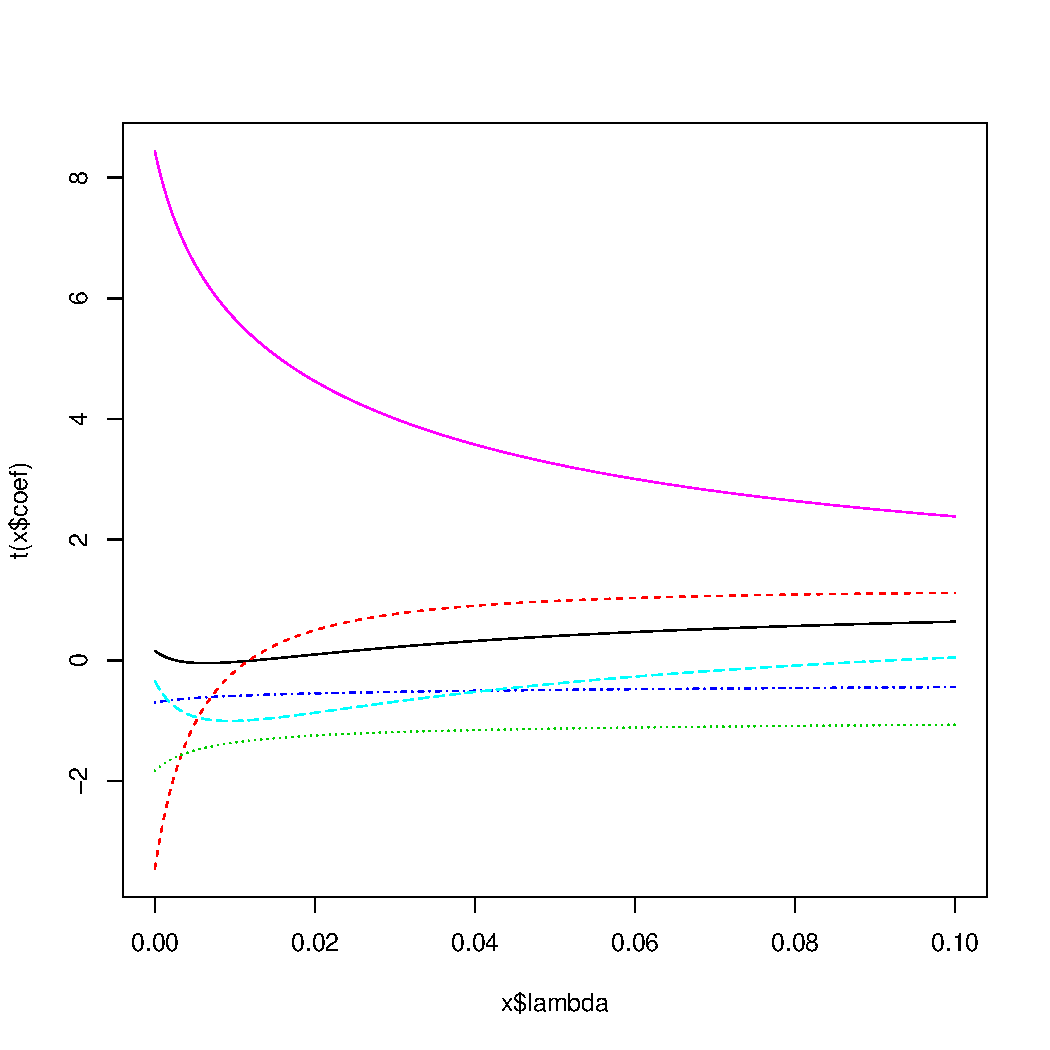
\includegraphics[height=3in]{ridge-trace}}
\end{frame}
\begin{frame}[fragile]
\frametitle{Generalized Cross-validation}
\begin{small}
\begin{verbatim}
> select(lm.ridge(Employed ~ ., data=longley, 
         lambda=seq(0, 0.1, 0.0001)))

modified HKB estimator is 0.004275357 
modified L-W estimator is 0.03229531 
smallest value of GCV  at 0.0028 

> longley.RReg = lm.ridge(Employed ~ ., data=longley, 
                          lambda=0.0028)
> coef(longley.RReg)
           GNP.deflator    GNP     Unemployed  Armed.Forces 
-2.950e+03 -5.381e-04   -1.822e-02  -1.76e-02 -9.607e-03 

 Population     Year 
-1.185e-01  1.557e+00 
\end{verbatim}
 
\end{small}

\end{frame}
\begin{frame} \frametitle{Shrinkage}
  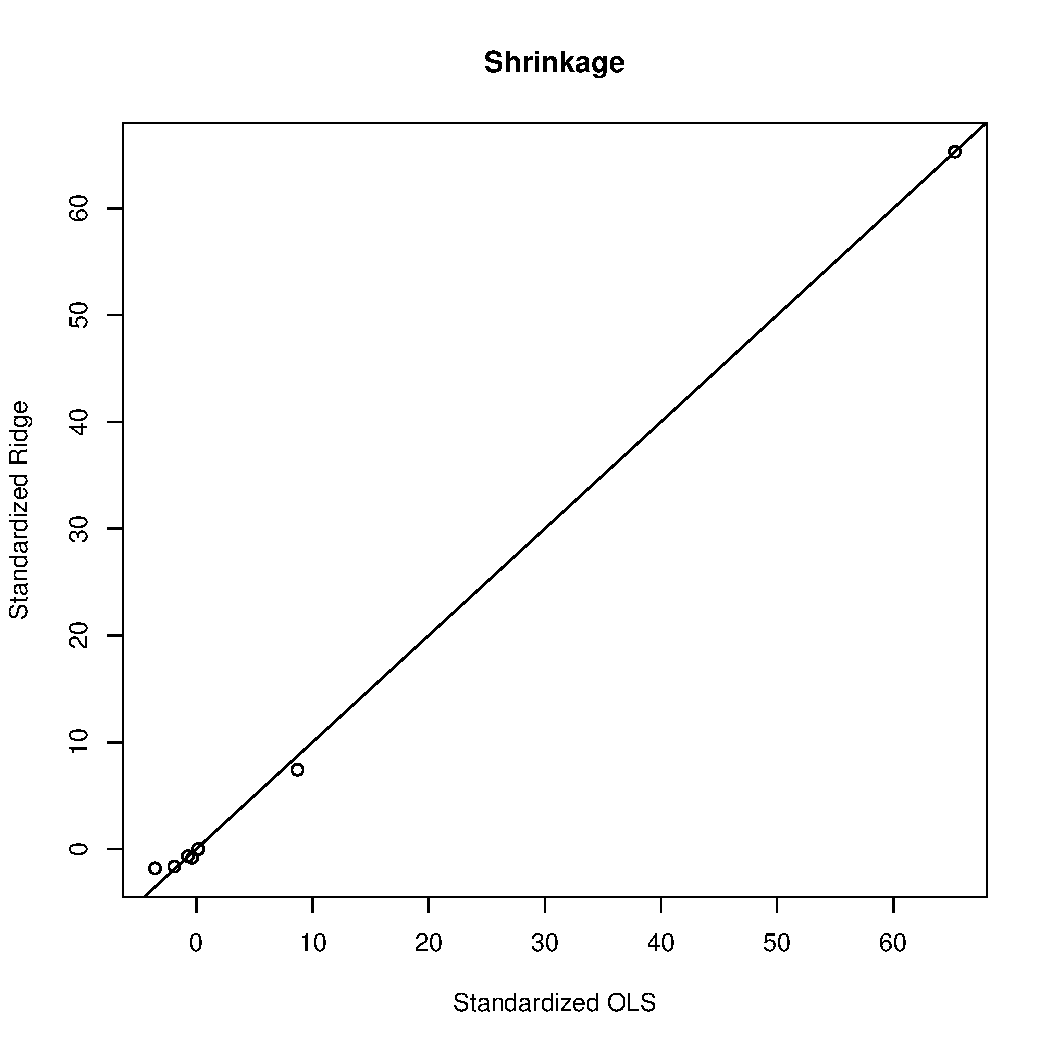
\includegraphics[height=3.5in]{shrinkage-ridge}
\end{frame}

\begin{frame}
  \frametitle{Bayesian Ridge: Prior on $k$}
  Reparameterization:
  \begin{eqnarray*}
  \Y  & =  &\one \alpha + (\I - \P_{\one}) \X S^{-1/2} S^{1/2} \b +
  \eps   \pause \\
      & = & \one \alpha + \X^s \b^s + \eps\\
 \Y^c & = & \X^s\b^s + \eps^s \qquad \eps^s \sim \N(\zero, (\I -
 \P_{1})/\phi) \pause \\
 \Ybar \mid \alpha, \phi & \sim & N(\alpha, 1/(n \phi)) \pause \\
 \U_{p} \Y & = &  L \g + \eps_p \qquad  \eps_p \sim \N(\zero,
 \I_p/\phi) \pause \\
\SSE \equiv \Y^T \U_{n-p-1} \U_{n-p-1}^T \Y  & \sim & \G( (n-p-1)/2, \phi/2)
  \end{eqnarray*}

Hierarchical prior \pause
\begin{itemize}
\item $p(\alpha \mid \phi, \g, \kappa) \propto 1$ \pause
\item $\g \mid \phi, \kappa \sim \N(\zero, \I (\phi \kappa )^{-1})$ \pause
\item $p(\phi \mid \kappa) \propto 1/\phi$
\item prior on $\kappa$?  Take $\kappa \mid \phi \sim  \G(1/2, 1/2)$ \pause
\end{itemize}
\end{frame}
\begin{frame}
  \frametitle{Posterior Distributions}
Joint Distribution
  \begin{itemize}
  \item $\alpha, \g, \phi \mid \kappa, \Y$  Normal-Gamma family given $\Y$
    and $\kappa$ \pause
  \item $\kappa \mid \Y$  not tractable \pause
  \end{itemize}
Obtain marginal for  $\g$ via  \pause
\begin{itemize}
\item Numerical integration \pause
\item MCMC:  Full conditionals \pause \\  Pick initial values $\alpha^{(0)}, \b^{(0)},
  \phi^{(0)}$, \pause \\
  Set  $t = 1$
  \begin{enumerate}
  \item Sample $\kappa^{(t)} \sim p(\kappa \mid \alpha^{(t-1)},
    \g^{(t-1)}, \phi^{(t-1)}, \Y)$ \pause
   \item Sample $\alpha^{(t)}, \g^{(t)}, \phi^{(t)} \mid \kappa(t),
     \Y$ \pause
 \item Set $t = t + 1$ and repeat until $t > T$ \pause
  \end{enumerate}
Use Samples  $\alpha^{(t)}, \g^{(t)}, \phi^{(t)}, \kappa^{(t)}$ for $t
= B, \ldots, T$ for inference \\
Change of variables to get back to $\b$
\end{itemize}
\end{frame}

\begin{frame}
\frametitle{Rao-Blackwellization Model}

What is ``best'' estimate of $\b$ from Bayesian perspective?
\begin{itemize}
\item  Loss  $(\b - \a)^T(\b - \a)$   under action $\a$
\item  Decision Theory:  Take action $\a$ that minimizes posterior
  expected loss which is posterior mean of $\b$.

\item Estimate of posterior mean is Ergodic average of MCMC:
  $\sum_i \b^{s(t)}/T \to $
\item Posterior mean given $\kappa$
  $$\tilde{\b^s}(\kappa) = (\X^{sT}\X^s + \kappa \I)^{-1}  \X^{sT}\X^s \bhat^s$$ \pause


\item Rao-Blackwell Estimate
  $$\frac{1}{T}\sum_t (\X^{sT}\X^s + \kappa^{(t)} \I)^{-1}  \X^{sT}\X^s \bhat^s$$ \pause


  \end{itemize}



\end{frame}

\begin{frame} \frametitle{Testimators}

Goldstein \& Smith (1974) have shown that if

\begin{enumerate}
\item
$0 \leq  h_i \leq 1$ and  $\tilde{\gamma}_i = h_i \hat{\gamma}_i$  
\item $\frac{\gamma^2_i}{\Var(\hat{\gamma}_i)} < \frac{1 + h_i}{1 - h_i}$
\end{enumerate}
then   $\tilde{\gamma}_i$ has smaller MSE than $\hat{\gamma}_i$

\vspace{14pt}
Case:  If $\gamma_j < \Var(\hat{\gamma}_i) = \sigma^2/l_i^2$  then
$h_i = 0$ and $\tilde{\gamma}_i$ is better.

\vspace{11pt}
Apply: Estimate $\sigma^2$ with SSE/(n - p - 1) and $\gamma_i$ with
$\hat{\gamma}_i$.  Set $h_i = 0$ if t-statistic is less than 1.
\vfill 
``testimator'' - see also Sclove (JASA 1968) and Copas ( JRSSB 1983)
\end{frame}
\begin{frame} \frametitle{Generalized Ridge}


Instead of $\gamma_j \simiid \N(0, \sigma^2/k)$ take 

$$\gamma_j \ind \N(0, \sigma^2/\kappa_i)$$  \pause

Then Condition of Goldstein \& Smith becomes

$$
\gamma_i^2 < \sigma^2\left[ \frac{2}{\kappa_j} + \frac{1}{l_i^2}  \right]
$$ \pause
\begin{itemize}
\item 
If $l_i$ is small almost any $\kappa_i$ will improve over OLS \pause
\item 
if $l_i^2$ is large then only very small values of $\kappa_i$ will give an
improvement \pause
\item Prior on $\kappa_i$?   \pause
\item Prior that can capture the feature above?

\end{itemize}

\end{frame}
\begin{frame}
  \begin{itemize}
\item Induced prior on $\b$?  
$$\gamma_j \mid \sigma^2, \kappa_j  \ind \N(0, \sigma^2/\kappa_j) \Leftrightarrow 
\b \sim \N(\zero, \sigma^2 \V\ \K^{-1} \V^T)$$
which is not diagonal.   
  \item  Or start with $$\b  \mid \sigma^2, \K \sim \N(0, \sigma^2 K)$$
 \item loss of invarince with linear transformations of $\X^s$
\item $\X^s \A \A^{-1} \b = \Z \alphav$ where $\A^{-1} \b = \alphav$
  \end{itemize}
\end{frame}
\begin{frame} \frametitle{Related Regression on PCA}
  \begin{itemize}
  \item 
  Principal Components of $\X$ may be obtained via the Singular Value
  Decomposition:  

$$\X = \U_p \L \V^T$$   
\pause
\item the $l_i$ are the eigenvalues of $\X^T\X$ \pause
  \begin{align*}
 \Y & = \one \alpha + \U \L \V^T \b + \eps  \\
    & = \one \alpha + \F \g + \eps \\ 
  \end{align*}
\item Columns $\F_i \propto \U_i$ are the principal components of the
  data multivariate data $\X_1, \ldots, \X_p$ \pause
\item If the direction $\F_i$ is ill-defined ($l_i = 0$  or $\l_i < \eps$
     then we may decide to not use $\F_i$ in the model.  \pause
\item equivalent to setting
  \begin{itemize}
  \item $\tilde{\gamma}_i = \hat{\gamma}_i$ if  $l_i\geq \eps$
  \item $\tilde{\gamma}_i = 0$ if  $l_i < \eps$ \pause
  \end{itemize}
  \end{itemize}
How to choose $\eps$?   Why should $\Y$ be related to first $k$
principal components?
\end{frame}
\begin{frame} \frametitle{Summary }

  \begin{itemize}
  \item OLS can clearly be dominated by other estimators for
    extimating $\b$  \pause
  \item Lead to Bayes like estimators \pause
  \item choice of penalties or prior hyper-parameters \pause
  \item hierarchical model with prior on $\kappa_i$ \pause
  \item Shrinkage, dimension reduction \& variable selection ? \pause
  \item what loss function?  Estimation versus prediction?  Copas 1983
  \end{itemize}

\end{frame}

\begin{frame} \frametitle{Full Conditionals}
  
\end{frame}

\begin{frame} \frametitle{Full Conditionals}
  
\end{frame}

\begin{frame} \frametitle{Full Conditionals}
   
\end{frame}

\end{document}

